\section{Analysis}
Here, first a statistical approach is taken to assess the accuracy of the MC model, before further testing different variations of inputs.
One thing to note, is that the data shortly after the indection dies out is cut for the MC solver. 
This is because ashortly fter the infection dies, the whole poulation becomes susceptible with no odds of getting infected.
In the RK solver however, infections never reach exactly zero, they only converge to the expected values, which makes this type of determinaiton less viable for the RK solver.
The RK solver may dip very close to zero infections, and then rise back up to some higher value. 
But, since the MC solver is discrete it infections, when 1 turns to 0, nothing more can happen.
Thus, if the MC data seem to cutoff early, it is only because nothing of interest happens after that point.

Another thing to note is that there are 15 inputs parameters that can affect the result of the model. 
So, it is absolutely not in the scope of this report to thoroughly check how every combination works.
There are probably combinations that should've or could've been tried, but to keep the report brief and concise, only some combinations and variations of each input parameter group is explored.
The main aim of this project is to develop two models for disease, and check that it can handle different inputs, not to map every single combination of inputs possible.
\subsection{Error and accuracy}
Before looking at any results, it is worth considering the error, and standard deviation in the results we see in the RK and MC solver.
The RK solve has error $O(h^5)$, whcich isn't really interesting to investigate further.
The MC solver however, does not have a pre-defined theoretical error, and as a result must be evaluated statistically.


In order to make results somewhat comparable, an attempt to keep the parameters the same as much as possible is made.
\begin{figure}[!h]
    \centering
    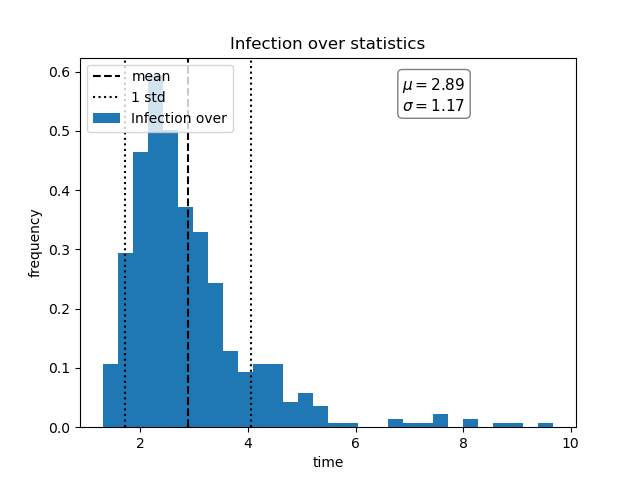
\includegraphics[scale=0.55]{plots/MC_solver_multiple_a_4_b_4_c_0.5500over_I500.png}
    \caption{Comparison of RK solver (dashed) and MC simulation (line) with expected values (horizontal dashed) with $a=4$, $b=4$ and $c=0.5$}
    \label{fig:error_Iover}
\end{figure}

In \textit{Figure} \ref{fig:error_Iover} and \ref{fig:error_Ipeak}, a simulation is ran with $a=4$, $b=4$ and $c=0.5$ 500 times, where we expect an initial peak of infections, before the infection dies out completely.
However, we see that the time of the infection peak, as well as the time of the infection being over, has $\sigma$ within the same order of magnitude as the mean.
This means that although the MC solver roughly does what you'd expect, there's a lot of random variety within each set of initial conditions.

\begin{figure}[!h]
    \centering
    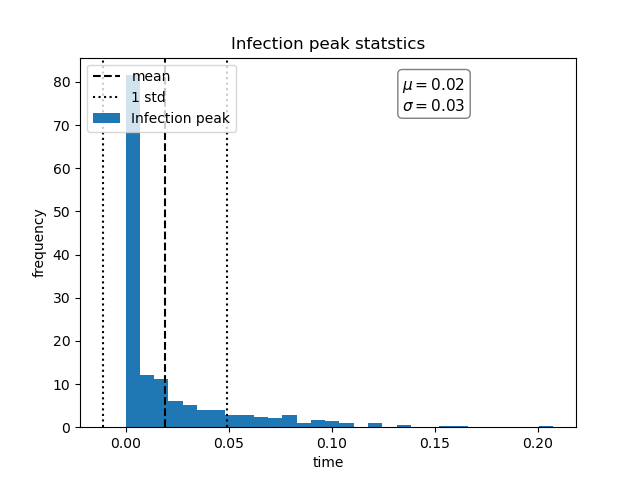
\includegraphics[scale=0.55]{plots/MC_solver_multiple_a_4_b_4_c_0.5500Peak_I500.png}
    \caption{Comparison of RK solver (dashed) and MC simulation (line) with expected values (horizontal dashed) with $a=4$, $b=4$ and $c=0.5$}
    \label{fig:error_Ipeak}
\end{figure}

In \textit{Figure} \ref{fig:error_meanI}, the mean value of the number of infections after reaching a steady state is calculated, and again we see significant variation. 
However, compared to infection peak and infection over as discussed above, the $\sigma$ value is roughly one order of magnitude lower than the mean. 

\begin{figure}[!h]
    \centering
    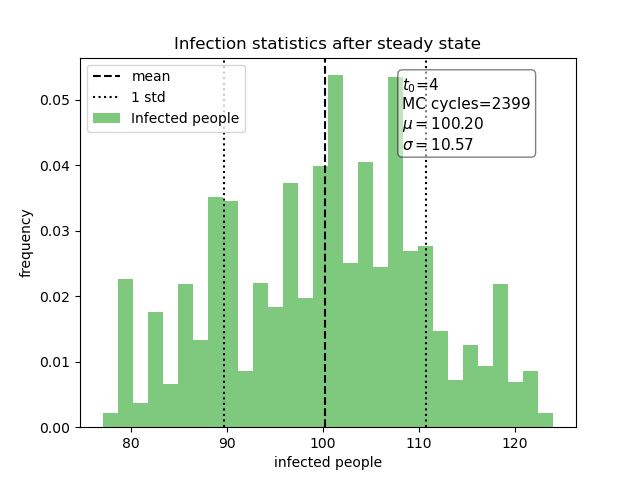
\includegraphics[scale=0.55]{plots/MC_solver_error_a_4_b_1_c_0.5I_SS_mcs_2399.png}
    \caption{Comparison of RK solver (dashed) and MC simulation (line) with expected values (horizontal dashed) with $a=4$, $b=4$ and $c=0.5$}
    \label{fig:error_meanI}
\end{figure}

In general, the MC solver has a lot of variety, yet it seems to do what it should within an order of magnitude of time. 
The variation after reaching the steady state seems be much lower, while still having quite a bit of random variation.

\subsection{The impact of changing b}
The first scenario to be considered, is with only $a$, $b$ and $c$.
To keep things simple, only b will change such that $b\in \{1,2,3,4\}$.
From the equations for expected values, we need $b<a$ in order for an infection to reach a steady state within a population.
\begin{figure}[!h]
    \centering
    \subfloat[]{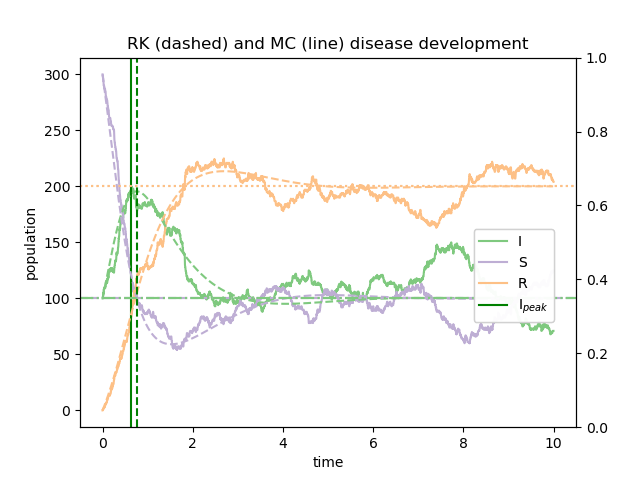
\includegraphics[scale=0.5]{plots/Compare_bbb_a_4_b_1_c_0.5.png}}
    \subfloat[]{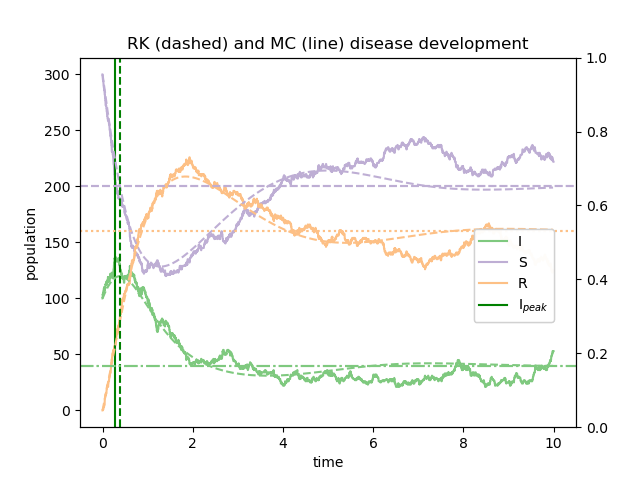
\includegraphics[scale=0.5]{plots/Compare_bbb_a_4_b_2_c_0.5.png}}\\
    \subfloat[]{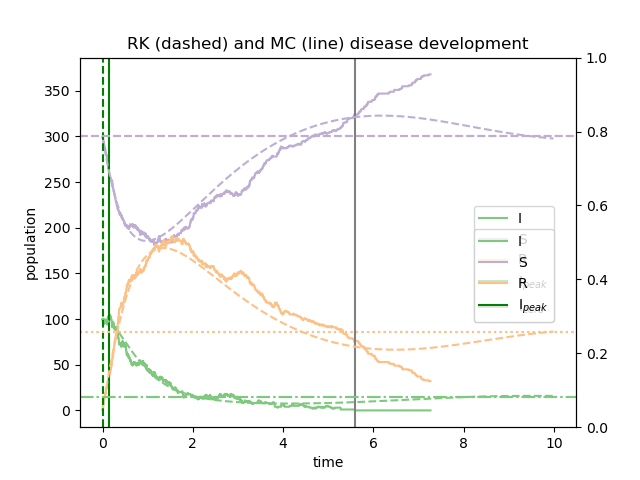
\includegraphics[scale=0.5]{plots/Compare_bbb_a_4_b_3_c_0.5.png}}
    \subfloat[]{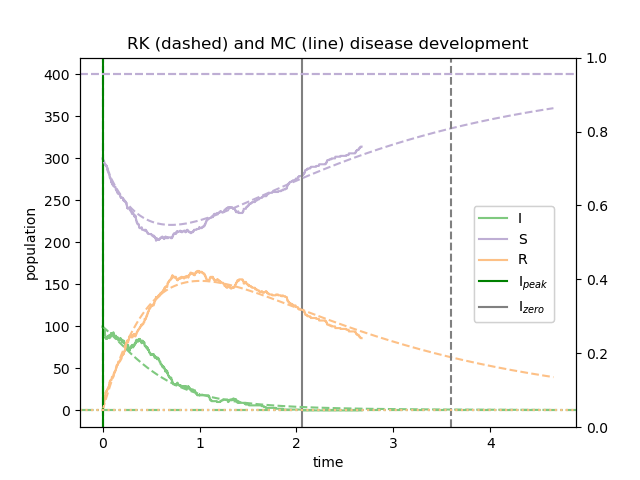
\includegraphics[scale=0.5]{plots/Compare_bbb_a_4_b_4_c_0.5.png}}
    \caption{Comparison of RK solver (dashed) and MC simulation (line) with expected values (horizontal dashed) with fixed $a=4$ and $c=0.5$. 
    $b$ has values 1(a), 2(b), 3(c) and 4(d). The horizontal dashed lines are the expected values.}
    \label{fig:b}
\end{figure}
In \textit{Figure} \ref{fig:b}, the RK and MC approach the expected values, and we see that the infection manages to reach steady state within the population for $b=1$ and $b=2$.
However, due to the randomness in the MC solver, as discussed above, the infection actually dies out in the run with $b=3$, due to the expected amount of infected people only being 14 at the steady state.
With a much larger population, this is expected to be less likely to happen. For $b=4$, the infection dies out as expected both for the MC and RK solver.

\subsection{Vital Parameters}
The next scenatio to be considered is including vital parameters narutal death $d$, natural birth $e$ and death due to disease $d_I$.
Having a ridiculously high birth rate or natural death rate doesn't really make any sense here, as it would either kill everyone or explode the population.
Ideally we want the population to be somewhat stable, and see how disease deaths influence the steady state of the system.
The key aspect here, is that when people die from the infection, it keeps them from infecting others, essentially killing the disease by removing carriers of the disease.
To explore this further, $e=0.011$ and $d=0.01$, while $d_I$ varies. 
Some key plots will be included to show how $d_I$ affects the steady state, and how fast the infection is over.


\begin{figure}
    \centering
    \subfloat[]{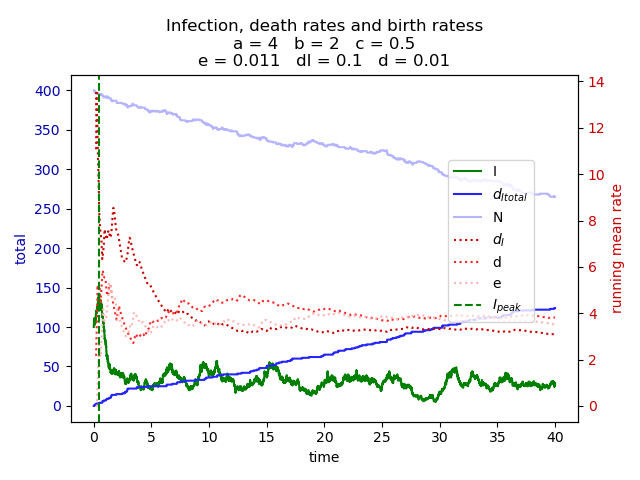
\includegraphics[scale=0.5]{plots/MC_solver_vital_a_4_b_2_c_0.5_IdI0.1.png}}
    \subfloat[]{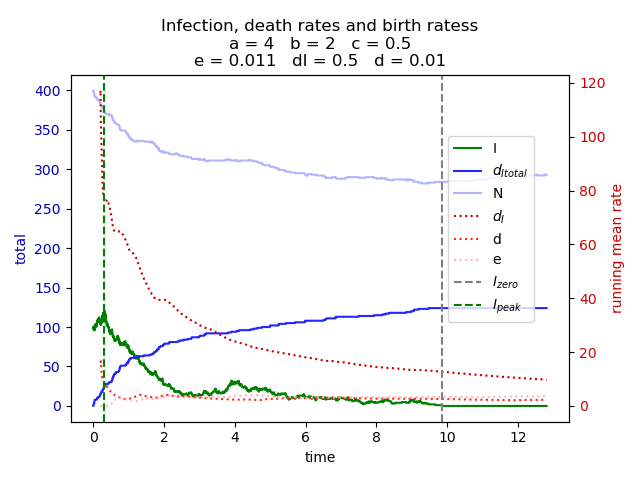
\includegraphics[scale=0.5]{plots/MC_solver_vital_a_4_b_2_c_0.5_IdI0.5.png}}\\
    \subfloat[]{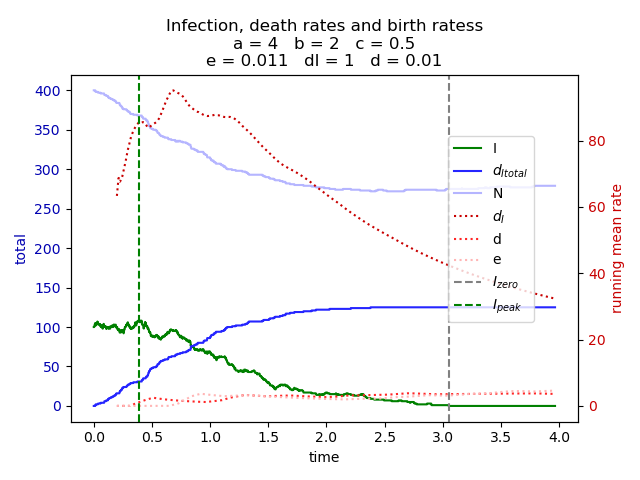
\includegraphics[scale=0.5]{plots/MC_solver_vital_a_4_b_2_c_0.5_IdI1.png}}
    \subfloat[]{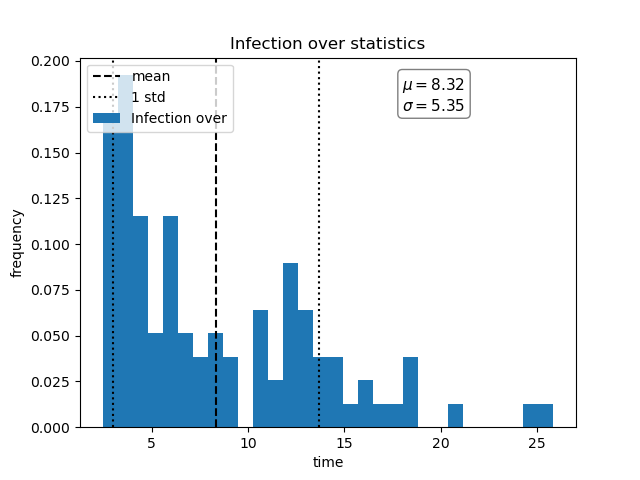
\includegraphics[scale=0.5]{plots/MC_solver_multiple_a_4_b_2_c_0.5100over_I100dI1.png}}
    \caption{Disease development for $a=4$, $b=2$, $c=0.5$, $e=0.011$ and $d=0.01$. $d_I$ varies as 0.1 (a), 0.5(b) and 1(c and d), with 100 runs collecting the statistics in (d)}
    \label{fig:vitalb2}
\end{figure}

In \textit{Figure} \ref{fig:vitalb2}, varying values of $d_I$ are shown for the previously stable case where $b=2$. 
However, with vital parameters introduced, we see that the disease ceases to be stable within the population, and eventually all the carriers are dead in the MC solver.
In the RK solver however, all the values converge to zero for $d_I=0.05$ and $d_I=0.1$, in contrast to the MC solver where the disease disappears.
In (d), we see that the MC simulation consistantly gets rid of the disease at approximately time = 20. 

To summarize, introducing disease deaths to a small population in the MC solver, causes the disease to go extinct faster, while also killing a lot of people.
However in the RK solver, the overall deathrate vs birthrate seems to dominate wether the population increases or converges to zero or some stable value.
In this case the RK solver is not really useful, as it seems to model disease porrly, and doesn't really model when there are no more infected left well.


In the case of the MC solver, having $d_I$ high actually causes the disease to die faster. To test this further, a smaller amount of initial infections are tested, to see if a high death rate actually prevents a disease to spread.
In \textit{Figure} \ref{fig:vitalI20} the initial infections are set to 20, but the disease development is still the same, just with a lower peak than before. 
This is due to the amount of susceptible people being so much higher when the infections are low, causing infections to grow even when the infection death rate is pretty high.
So, the death rate does not really seem to determine whether an infetion will die "early", only how fast it might make the disease extinct due to carriers dying after the infection peak.
\begin{figure}[!h]
    \centering
    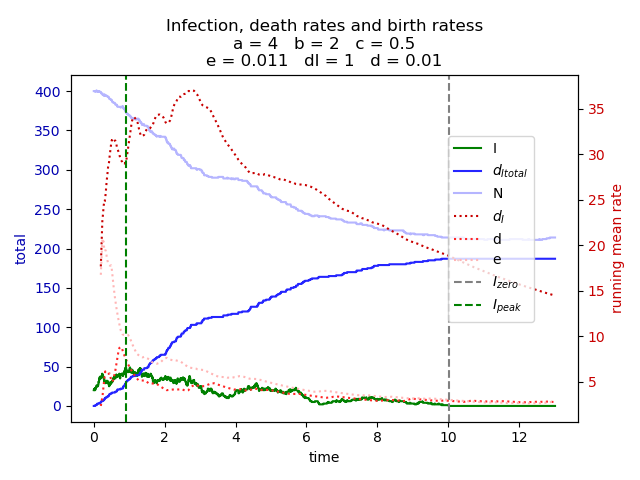
\includegraphics[scale=0.55]{plots/MC_solver_vitalI20_a_4_b_2_c_0.5_IdI1.png}
    \caption{A run with initial infections = 20, with $a=4$, $b=2$, $c=0.5$, $e=0.011$, $d=0.01$ and $d_I=1$.}
    \label{fig:vitalI20}
\end{figure}


\subsection{Seasonal Variation}
Another parameter that impacts things like the flu in particular, is seasonal variations.
To simulate this, the rate of infection $a_{seasonal}$ is modyfied by
$$
a_{seasonal}=a+Acos(\omega t)
$$
The average value of $a$ over a period $\omega k$, $k \in \mathbf{N} ^+$ remains unchanged, so does this mean that the amount of infected people also remain the same?
To explore this, $\omega = 2 \pi$, and $A \in \{1,2,3,4\}$ for $a=4$, $b=2$ or $b=1$ and $c=0.5$. Initially, no vital parameters will be introduced.

\begin{figure}
    \centering
    \subfloat[]{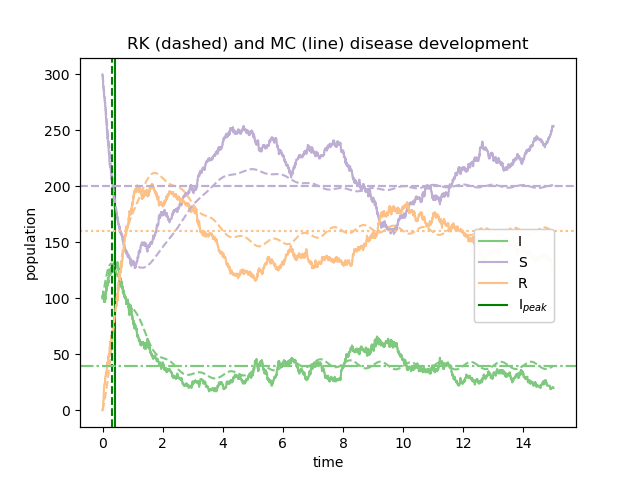
\includegraphics[scale=0.5]{plots/Compare_seasonalA1_a_4_b_2_c_0.5.png}}
    \subfloat[]{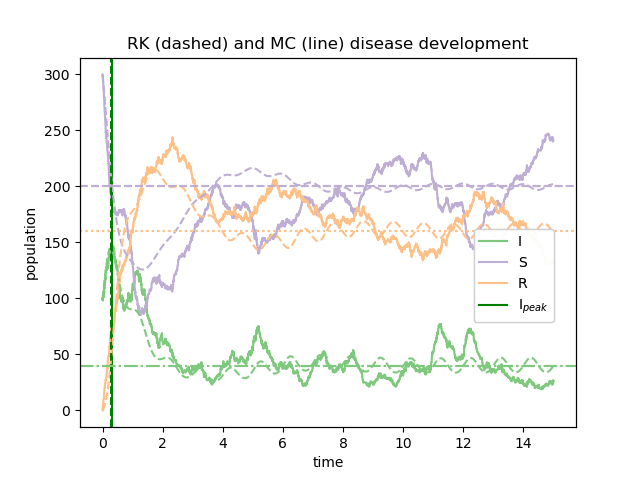
\includegraphics[scale=0.5]{plots/Compare_seasonalA2_a_4_b_2_c_0.5.png}}\\
    \subfloat[]{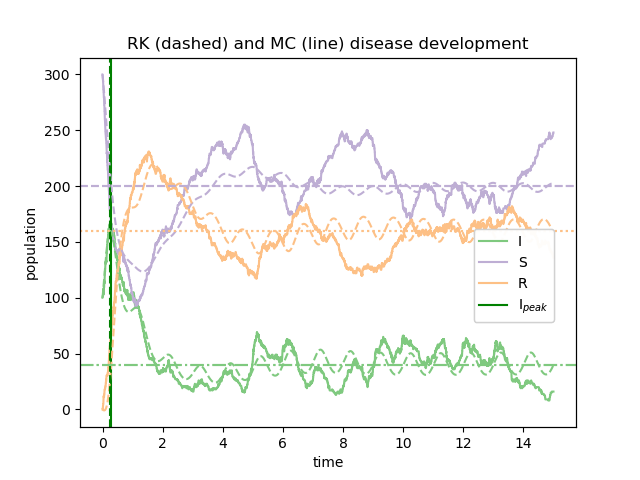
\includegraphics[scale=0.5]{plots/Compare_seasonalA3_a_4_b_2_c_0.5.png}}
    \subfloat[]{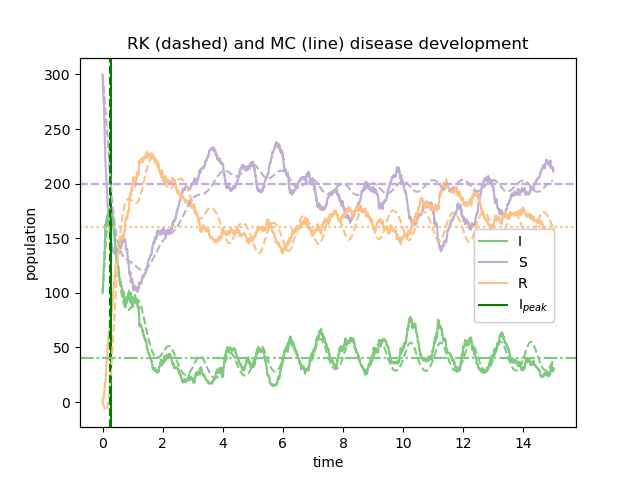
\includegraphics[scale=0.5]{plots/Compare_seasonalA4_a_4_b_2_c_0.5.png}}
    \caption{Disease development for $a=4$, $b=2$, $c=0.5$, with seasonal variation amplitude $A \in \{1,2,3,4\}$.}
    \label{fig:seasonalb2}
\end{figure}

Changing $b$ so that $b=1$ causes the expected values to for $I$ and $S$ to be the same, highlighting the cyclic relationship of the two, as seen in In \textit{Figure} \ref{fig:seasonalb1}

\begin{figure}
    \centering
    \subfloat[]{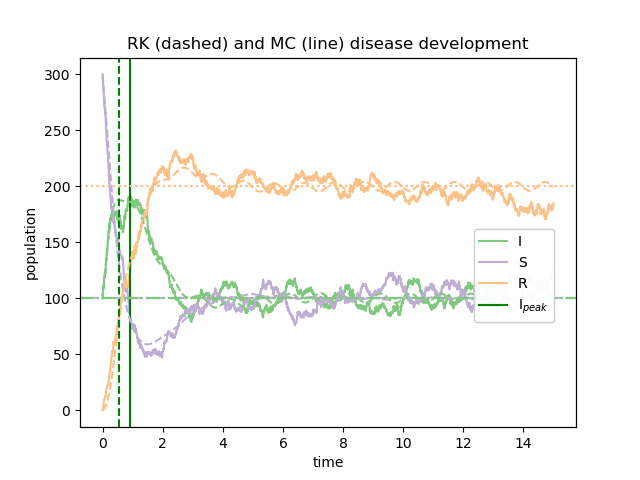
\includegraphics[scale=0.5]{plots/Compare_seasonalA1_a_4_b_1_c_0.5.png}}
    \subfloat[]{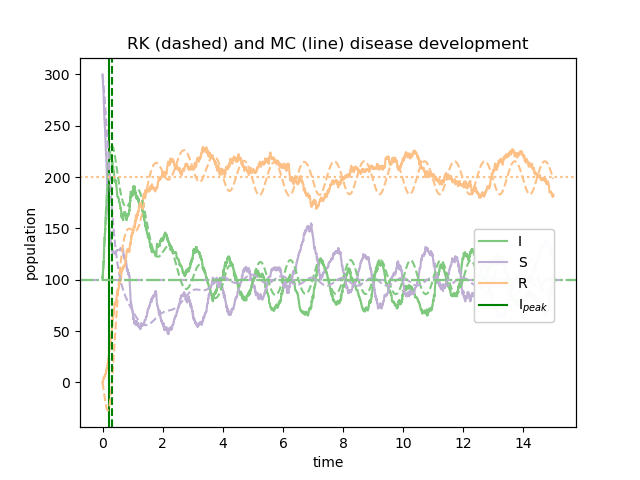
\includegraphics[scale=0.5]{plots/Compare_seasonalA4_a_4_b_1_c_0.5.png}}
    \caption{Disease development for $a=4$, $b=1$, $c=0.5$, with seasonal variation amplitude $A \in \{1,4\}$.}
    \label{fig:seasonalb1}
\end{figure}

So how does this affect the statistics of when an infection is over, or the mean amount of infected people?

\begin{figure}
    \centering
    \subfloat[]{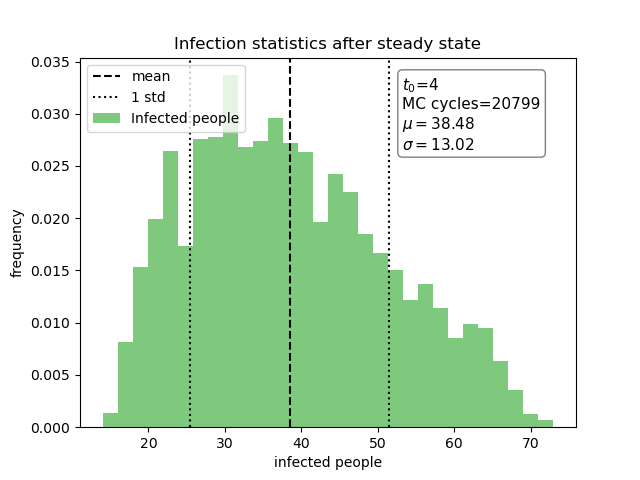
\includegraphics[scale=0.5]{plots/MC_solver_seasonalA4_a_4_b_2_c_0.5I_SS_mcs_2079920798.png}}
    \subfloat[]{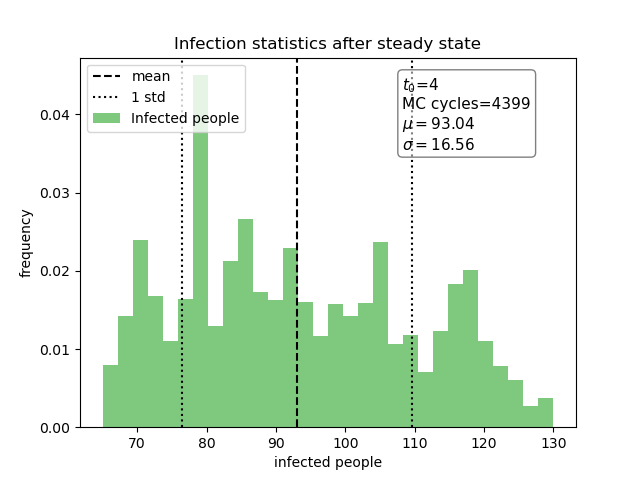
\includegraphics[scale=0.5]{plots/MC_solver_seasonalA4_a_4_b_1_c_0.5I_SS_mcs_43994398.png}}
    \caption{Disease statistics for Infections after steady state for $a=4$, $b=1$ (a) and $b=2$ (b), $c=0.5$, with seasonal variation amplitude $A = 4$.}
    \label{fig:seasonalb1}
\end{figure}

\begin{figure}
    \centering
    \subfloat[]{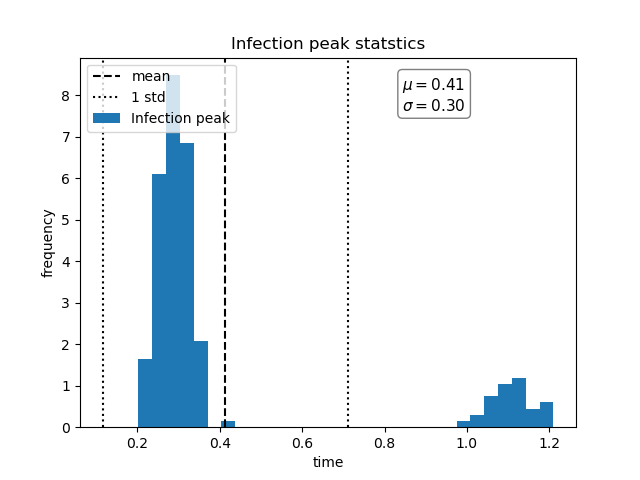
\includegraphics[scale=0.5]{plots/MC_solver_multiple_a_4_b_1_c_0.5200Peak_I200.png}}
    \subfloat[]{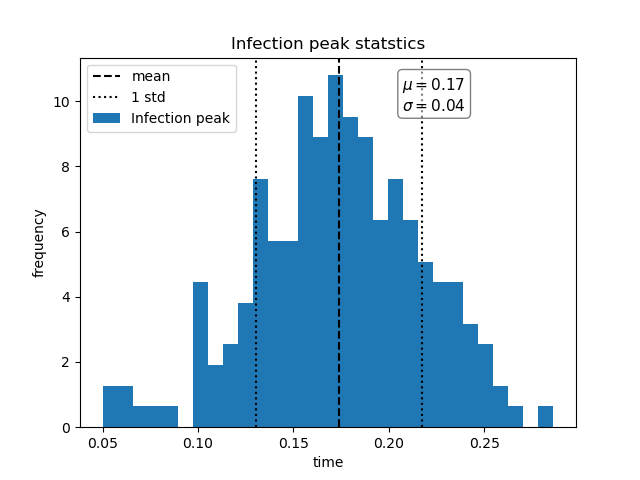
\includegraphics[scale=0.5]{plots/MC_solver_multiple_a_4_b_2_c_0.5200Peak_I200.png}}
    \caption{Infection peak for $a=4$, $b=1$ (a) and $b=2$ (b), $c=0.5$, with seasonal variation amplitude $A = 4$, and vital parameters $e=0.011$, $d=0.01$ and $d_I=1$ collecting statistics over 200 runs.}
    \label{fig:seasonalI_peak}
\end{figure}s


\begin{figure}
    \centering
    \subfloat[]{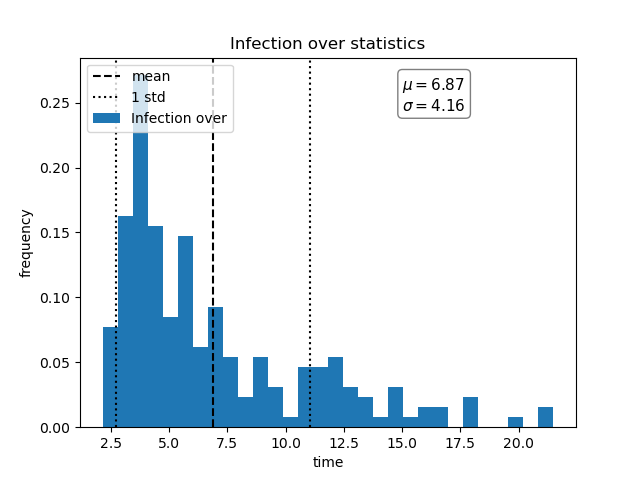
\includegraphics[scale=0.5]{plots/MC_solver_multiple_a_4_b_2_c_0.5200over_I200.png}}
    \caption{Infection over for $a=4$, $b=2$ (b), $c=0.5$, with seasonal variation amplitude $A = 4$, and vital parameters $e=0.011$, $d=0.01$ and $d_I=1$ collecting statistics over 200 runs.}
    \label{fig:seasonalI_over}
\end{figure}



\subsection{Vaccines}

\begin{figure}
    \centering
    \subfloat[]{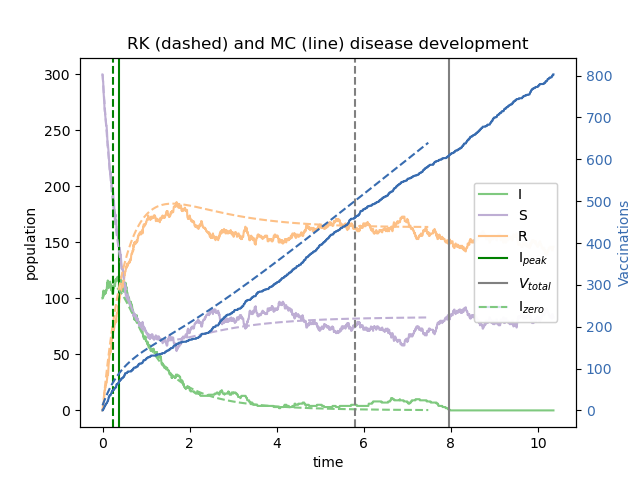
\includegraphics[scale=0.5]{plots/Compare_vaccines_a_4_b_1_c_0.5_f_1.png}}
    \subfloat[]{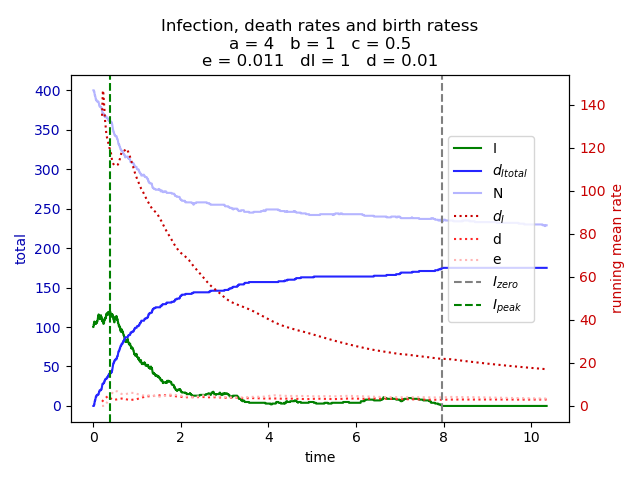
\includegraphics[scale=0.5]{plots/MC_solver_vaccines_a_4_b_1_c_0.5_f_1_IdI.png}}\\
    \subfloat[]{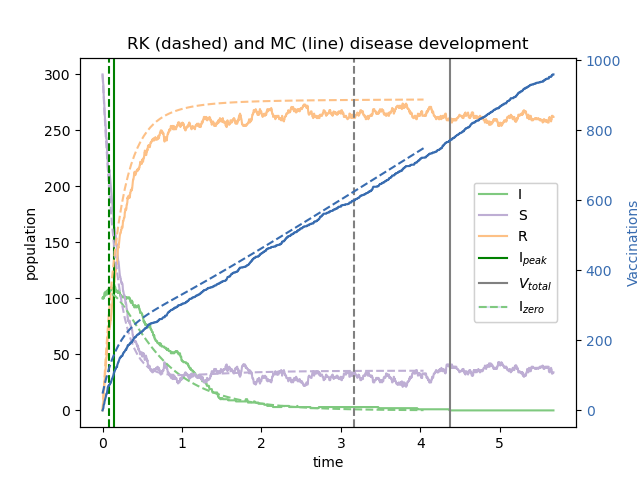
\includegraphics[scale=0.5]{plots/Compare_vaccines_a_4_b_1_c_0.5_f_4.png}}
    \subfloat[]{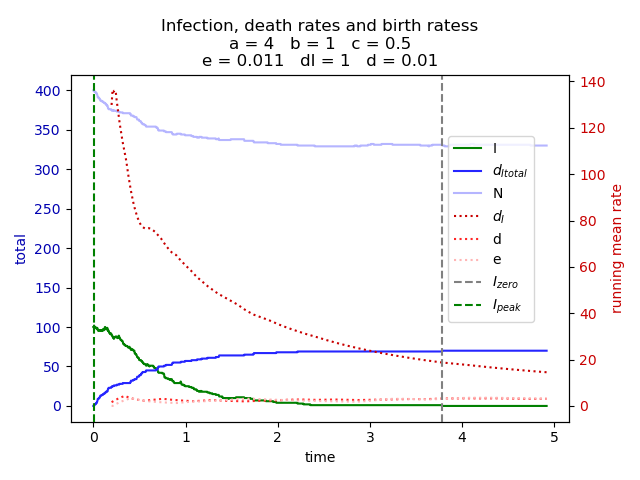
\includegraphics[scale=0.5]{plots/MC_solver_vaccines_a_4_b_1_c_0.5_f_8_IdI.png}}
    \caption{Disease development for $a=4$, $b=1$, $c=0.5$, with vaccination rates $f=1$ (a and b) and $f=8$ (c and d)}
    \label{fig:latevacc}
\end{figure}


\begin{figure}
    \centering
    \subfloat[]{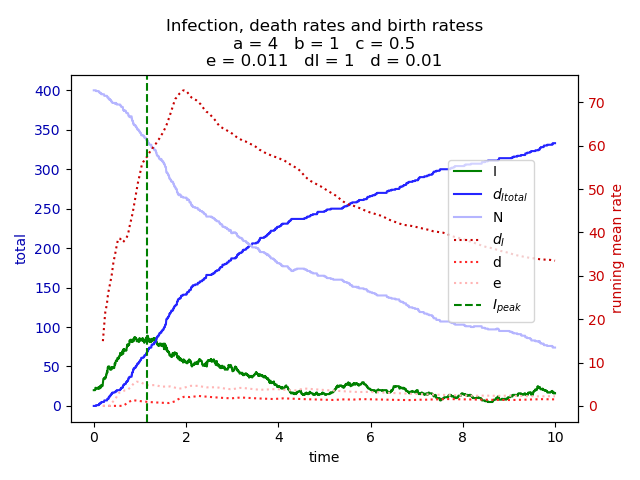
\includegraphics[scale=0.5]{plots/MC_solver_vaccinesI20_a_4_b_1_c_0.5_IdI.png}}
    \subfloat[]{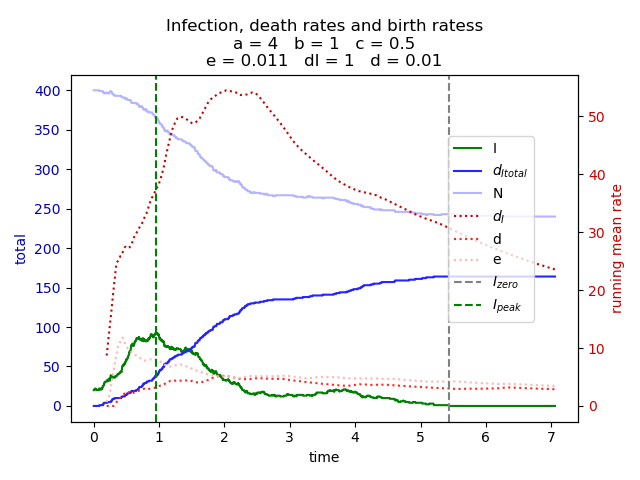
\includegraphics[scale=0.5]{plots/MC_solver_vaccinesI20_a_4_b_1_c_0.5_f_0.5_IdI.png}}\\
    \subfloat[]{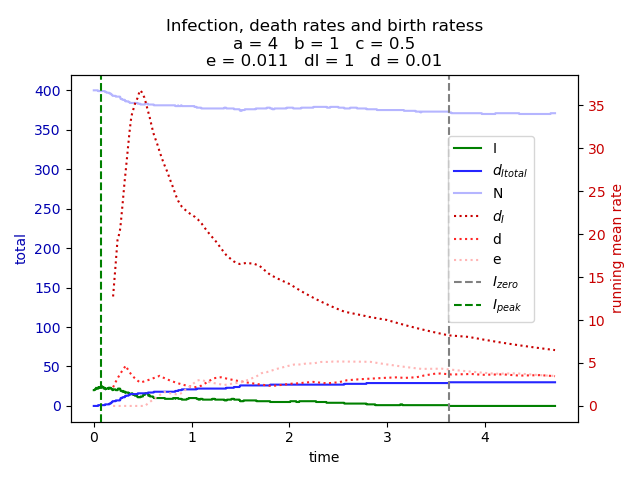
\includegraphics[scale=0.5]{plots/MC_solver_vaccinesI20_a_4_b_1_c_0.5_f_1_IdI.png}}  
    \subfloat[]{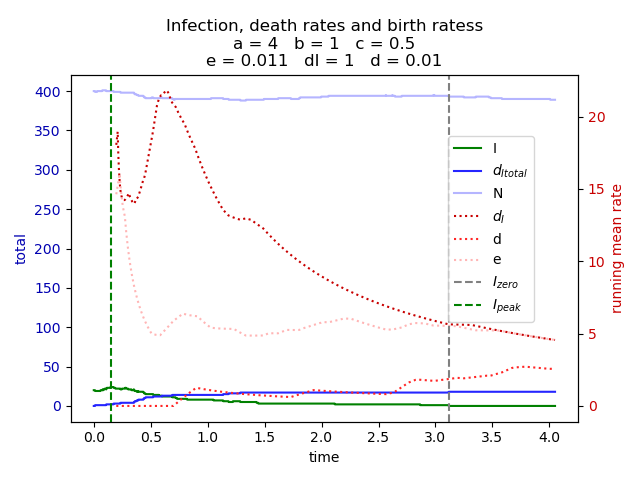
\includegraphics[scale=0.5]{plots/MC_solver_vaccinesI20_a_4_b_1_c_0.5_f_4_IdI.png}}
    \caption{Vaccination rates effect on disease development for $a=4$, $b=1$, $c=0.5$, with vaccination rates $f=0$ (a), $f=0.5$ (b), $f=1$ (a), $f=4$ (a)}
    \label{fig:earlyvacc}
\end{figure}
